\documentclass[a4paper, 12pt]{article}

\usepackage[T2A]{fontenc}
\usepackage[utf8]{inputenc}
\usepackage[english,russian]{babel}
\usepackage[left=15mm, top=20mm, right=15mm, bottom=20mm, nohead, nofoot]{geometry}

\usepackage{hyperref}
\usepackage{graphicx}
\usepackage{wrapfig}
\usepackage{afterpage}
\usepackage{amsmath, amsfonts, amssymb, amsthm, mathtools}
\author{Хомутов Андрей, группа Б06-903}
\title{ВПВ по курсу "Электричество и магнетизм" \\ Конденсатор на высоких частотах}
\date{22 декабря 2020 г.}
%%%%%%%%%%%%%%%%%%%%%%%%%%%%%%%%%%%%%%%%%%%%%%%%%%%%%%%%%%%%%%%%%%%%%%%%%
\usepackage{graphicx, wrapfig, subcaption, setspace, booktabs}
\usepackage[protrusion=true, expansion=true]{microtype}
\usepackage[english]{babel}
\usepackage{sectsty}
\usepackage{url, lipsum}
\newcommand{\HRule}[1]{\rule{\linewidth}{#1}}
\onehalfspacing
\setcounter{tocdepth}{5}
\setcounter{secnumdepth}{5}
%%%%%%%%%%%%%%%%%%%%%%%%%%%%%%%%%%%%%%%%%%%%%%%%%%%%%%%%%%%%%%%%%%%%%%%%%


\begin{document}

\title{ \normalsize \textsc{Лабораторная работа}
		\\ [4.0cm]
		\HRule{0.5pt} \\ [0.3cm]
		\LARGE \textbf{{Дифракция на ультразвуке}}
		\HRule{0.5pt} \\ [0.1cm]
		\normalsize  \vspace*{18\baselineskip}}

\date{}

\author{%Шамарина Екатерина, Б06-903 \\
		Хомутов Андрей, Б06-903 \\
ФБМФ, 2021\\ }

\maketitle
\thispagestyle{empty}
\newpage
%%%%%%%%%%%%%%%%%%%%%%%%%%%%%%%%%%%%%%%%%%%%%%%%%%%%%%%%%%%%%%%%%%%%%%%%%
\section*{Цели работы} 
\begin{enumerate}
    \item Изучение дифракции света на синусоидальной акустической решетке 
    \item Наблюдение фазовой решетки методом темного поля
\end{enumerate}
%%%%%%%%%%%%%%%%%%%%%%%%%%%%%%%%%%%%%%%%%%%%%%%%%%%%%%%%%%%%%%%%%%%%%%%%%
 
%\section{Теоретическая часть}
%\subsection{...}

%\subsubsection{...}


\section{Практическая часть}
\subsection{Определение скорости ультразвука по дифракционной картине}
После получения дифракционной картины на УЗ, определяется положение дифракционных полос. Результаты представлены в таблице 1. На рисунке 1 представлены зависимости координаты полосы от ее номера относительно центральной. По наклону графика можем определить расстояние между полосами:
\begin{itemize}
    \item Для частоты 1 МГц - $134 \pm 7$ мкм
    \item Для частоты 1.3 МГц - $161 \pm 2$ мкм
    \item Для частоты 2 МГц - $250 \pm 7$ мкм
    \item Для частоты 4.3 МГц - $532 \pm 3$ мкм
\end{itemize}
\begin{table}[h]
\begin{center}
\caption{Координаты полос на разных частотах}
\begin{tabular}{|c|c|c|}
\hline
Частота, МгГц        & Полоса & координата, 4мкм \\ \hline
\multirow{}{}{1,3} & -2     & 224              \\ \cline{2-3} 
                     & -1     & 180              \\ \cline{2-3} 
                     & 0      & 142              \\ \cline{2-3} 
                     & 1      & 101              \\ \cline{2-3} 
                     & 2      & 62               \\ \hline
\multirow{}{}{2}   & -1     & 210              \\ \cline{2-3} 
                     & 0      & 150              \\ \cline{2-3} 
                     & 1      & 85               \\ \hline
\multirow{}{}{4,3} & -1     & 279              \\ \cline{2-3} 
                     & 0      & 146              \\ \cline{2-3} 
                     & 1      & 13               \\ \hline
\multirow{}{}{1}   & -2     & 220              \\ \cline{2-3} 
                     & -1     & 178              \\ \cline{2-3} 
                     & 0      & 145              \\ \cline{2-3} 
                     & 1      & 114              \\ \cline{2-3} 
                     & 2      & 85               \\ \hline
\end{tabular}
\end{center}
\end{table}
\begin{figure}[h!]
    \begin{center}
    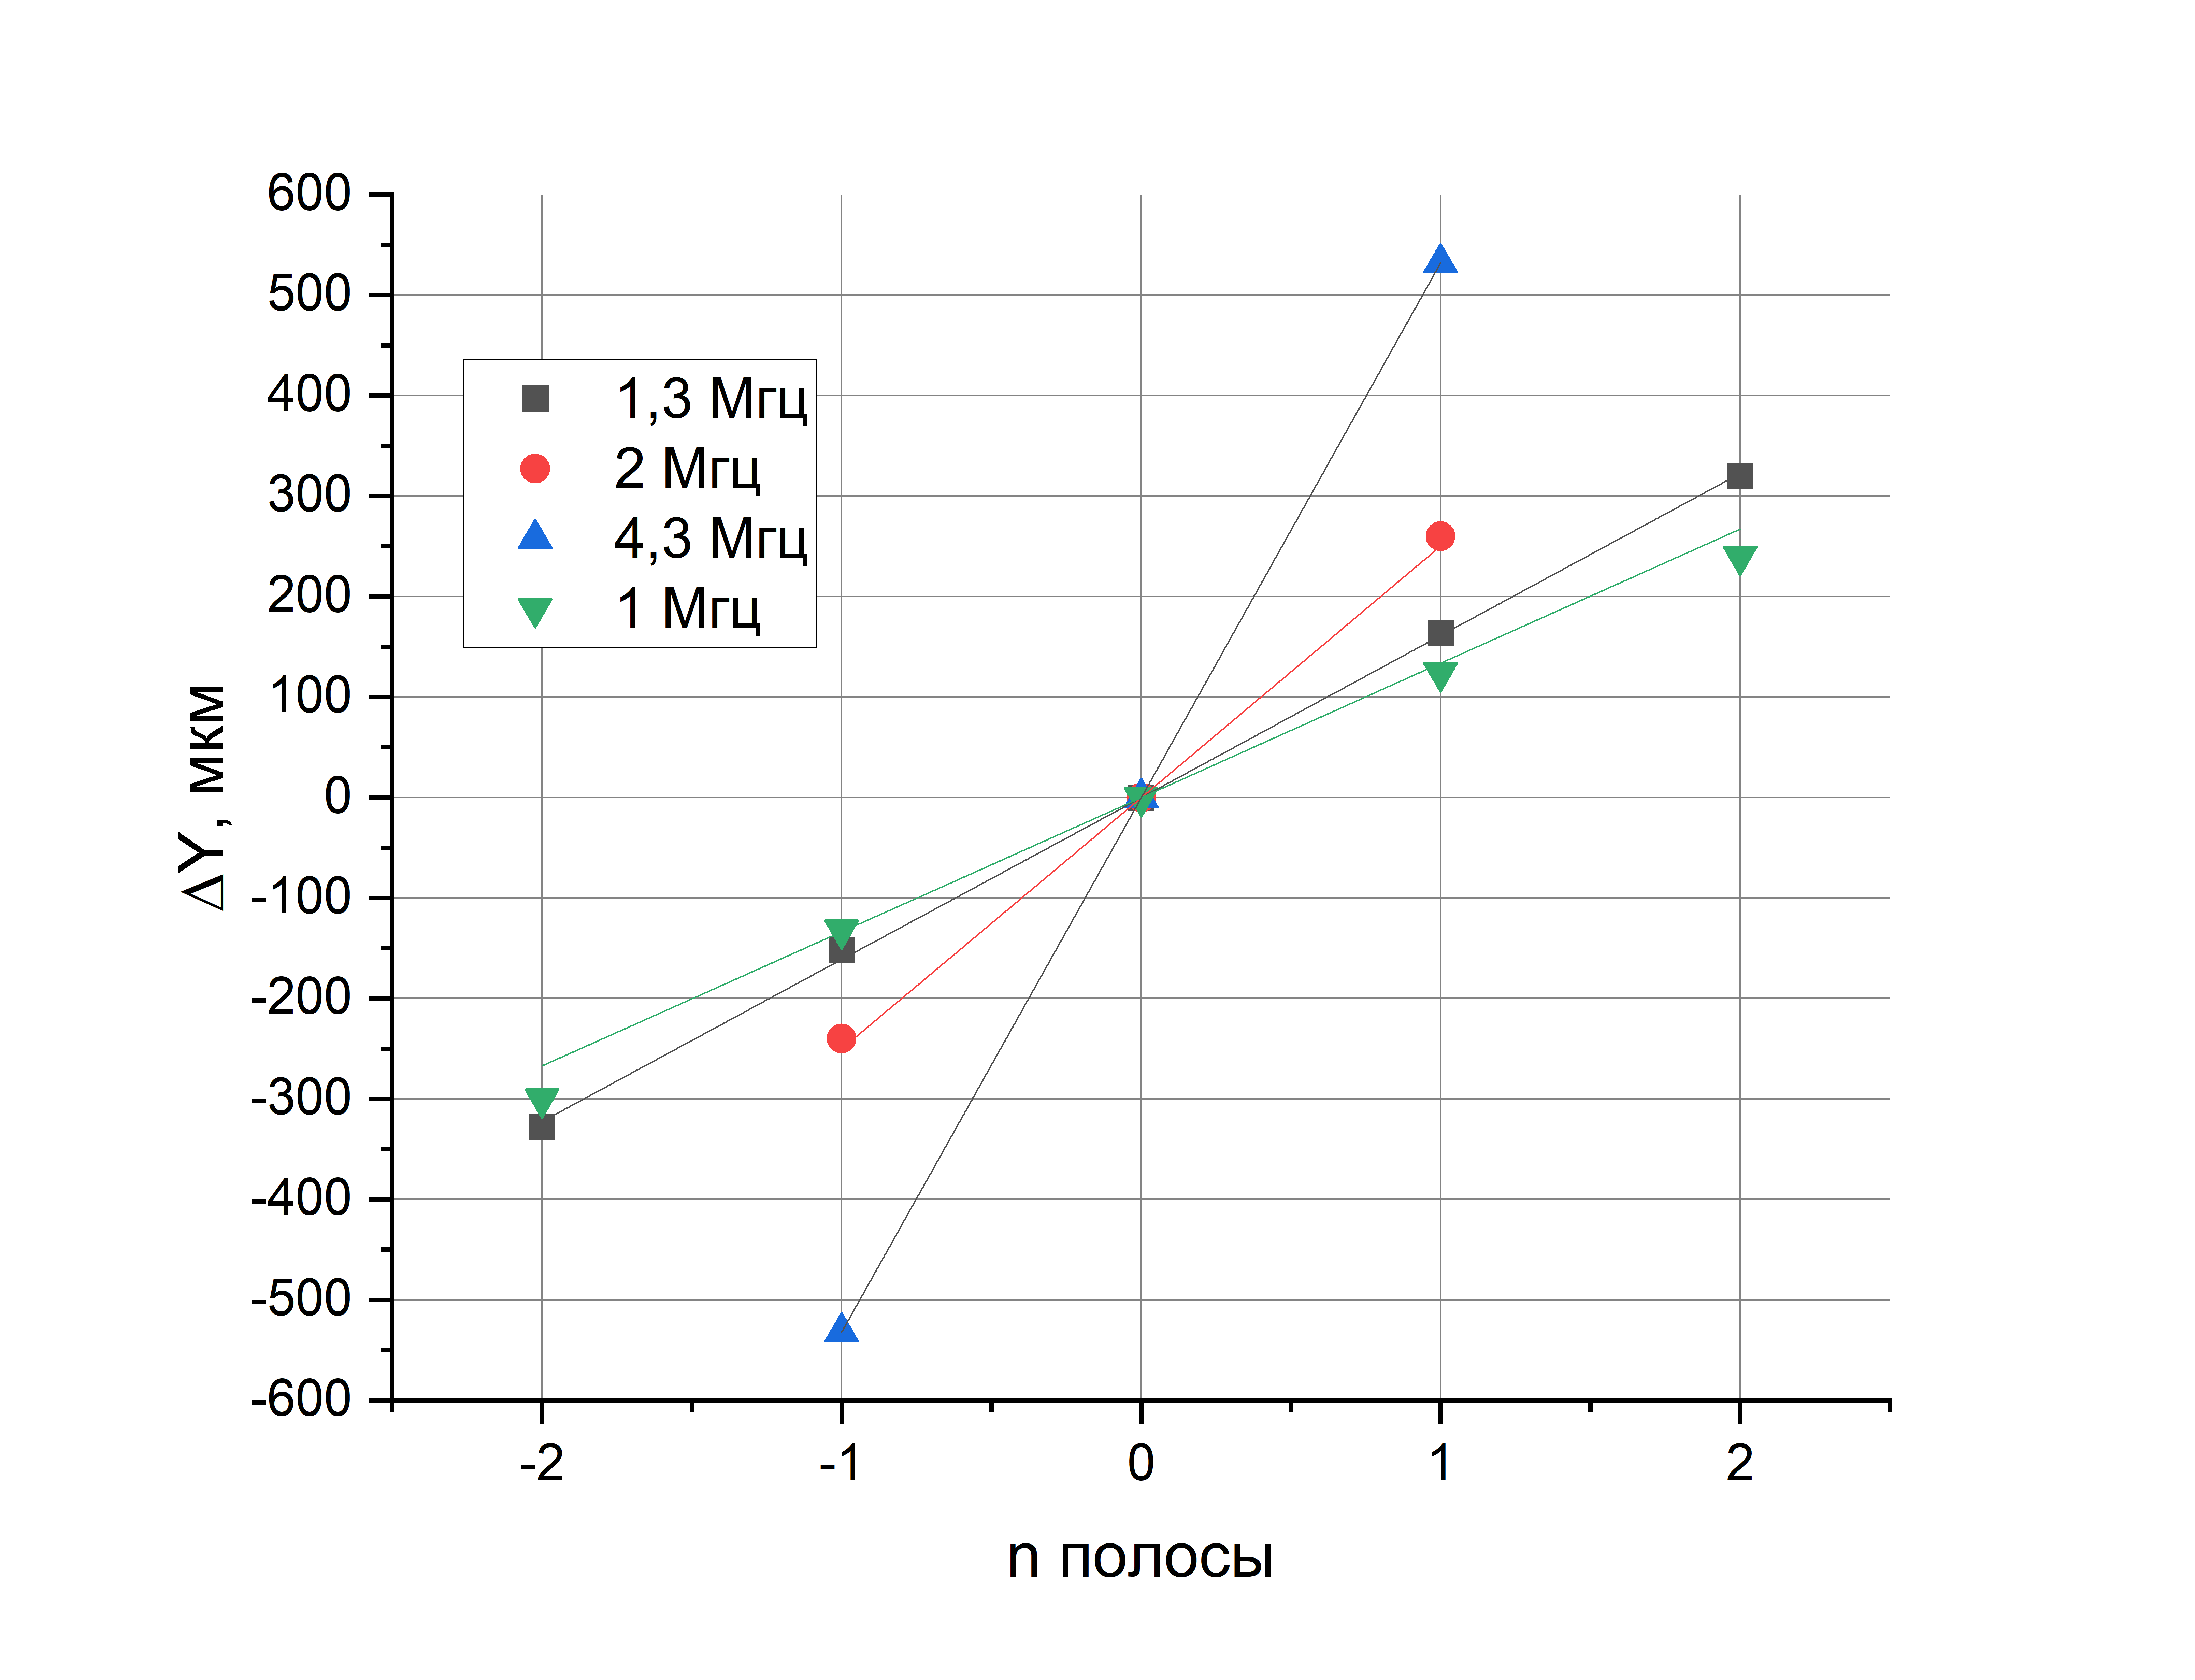
\includegraphics[width=0.8\textwidth]{lanes.png}
    \end{center}
    \caption{Длина волны от обратной частоты}
\end{figure}
Зная фокусное расстояние, рассчитывается длины волны как $\Lambda=\frac{mf\lamda}{l_{m}}$, где $f$ - фокусное расстояние объектива, равное 28см, $\lamda$ - длина волны ($6400\pm200$ ангстрем для красного светофильтра). Результаты расчетной длины волны и скорости представлены в таблице 2. Как видно, скорость звука совпадает с ожидаемыми 1400 м/с. Длина звуковой волны частоты порядка 1 МГц будет соствалять в воде порядка 1мм. 

\begin{table}[h]
\begin{center}
\caption{Скорость и длина волны}
\begin{tabular}{|c|c|c|c|c|c|c|}
\hline
    & $l_{m}/m$, мкм & $\delta(l_{m}/m)$, мкм & $\Lambda$, мм    & $\delta(\Lambda)$, мм   & $V$, м/с    & $\delta(V)$, м/с  \\ \hline
1   & 134  & 7 & 1,34 & 0,11 & 1337 & 110 \\ \hline
1,3 & 161  & 2 & 1,11 & 0,05 & 1447 & 60  \\ \hline
2   & 250  & 7 & 0,72 & 0,04 & 1434 & 90  \\ \hline
4,3 & 532  & 3 & 0,34 & 0,01 & 1448 & 50  \\ \hline
\end{tabular}
\end{center}
\end{table}
\subsection{Определение скорости ультразвука методом темного поля}
Закрыв нулевой дифракционный максимум, получаем фазовое изображение решетки, наблюдаемое в микроскоп. После калибровки микроскопа на миллиметровой решетке, определяем что на 2.5 единиц шкалы окуляра приходится 6мм объекта. 

Измеренное расстояние между n-ым количеством полос представлено в таблице 3. Тут же расчетная длина волны звука. Погрешность определения координаты - 0.05 ед. шкалы окуляра, определяется толщиной и размытостью изображений полос.
\begin{table}[h]
\begin{center}
\caption{Длина волны методом темного поля}
\begin{tabular}{|c|c|c|c|c|}
\hline
Частота, МГц & x1, дел & x2, дел & n  & $\Lambda$, мм \\ \hline
2            & 0,6     & 2,5     & 12 & 0,76      \\ \hline
1,69         & 1,64    & 0,47    & 8  & 0,70      \\ \hline
1,14         & 2,85    & 0,95    & 7  & 1,30      \\ \hline
1,04         & 2,85    & 1,05    & 6  & 1,44      \\ \hline
0,988        & 0,95    & 3,12    & 7  & 1,49      \\ \hline
1,34         & 1,1     & 2,5     & 6  & 1,12      \\ \hline
\end{tabular}
\end{center}
\end{table}

Построив график зависимости $\Lambda=F(1/\nu)$ (рис. 2) определяется скорость звуковых волн в воде $v_{\text{зв}} = 1440 \pm 150$ м/с.

\begin{figure}[h!]
    \begin{center}
    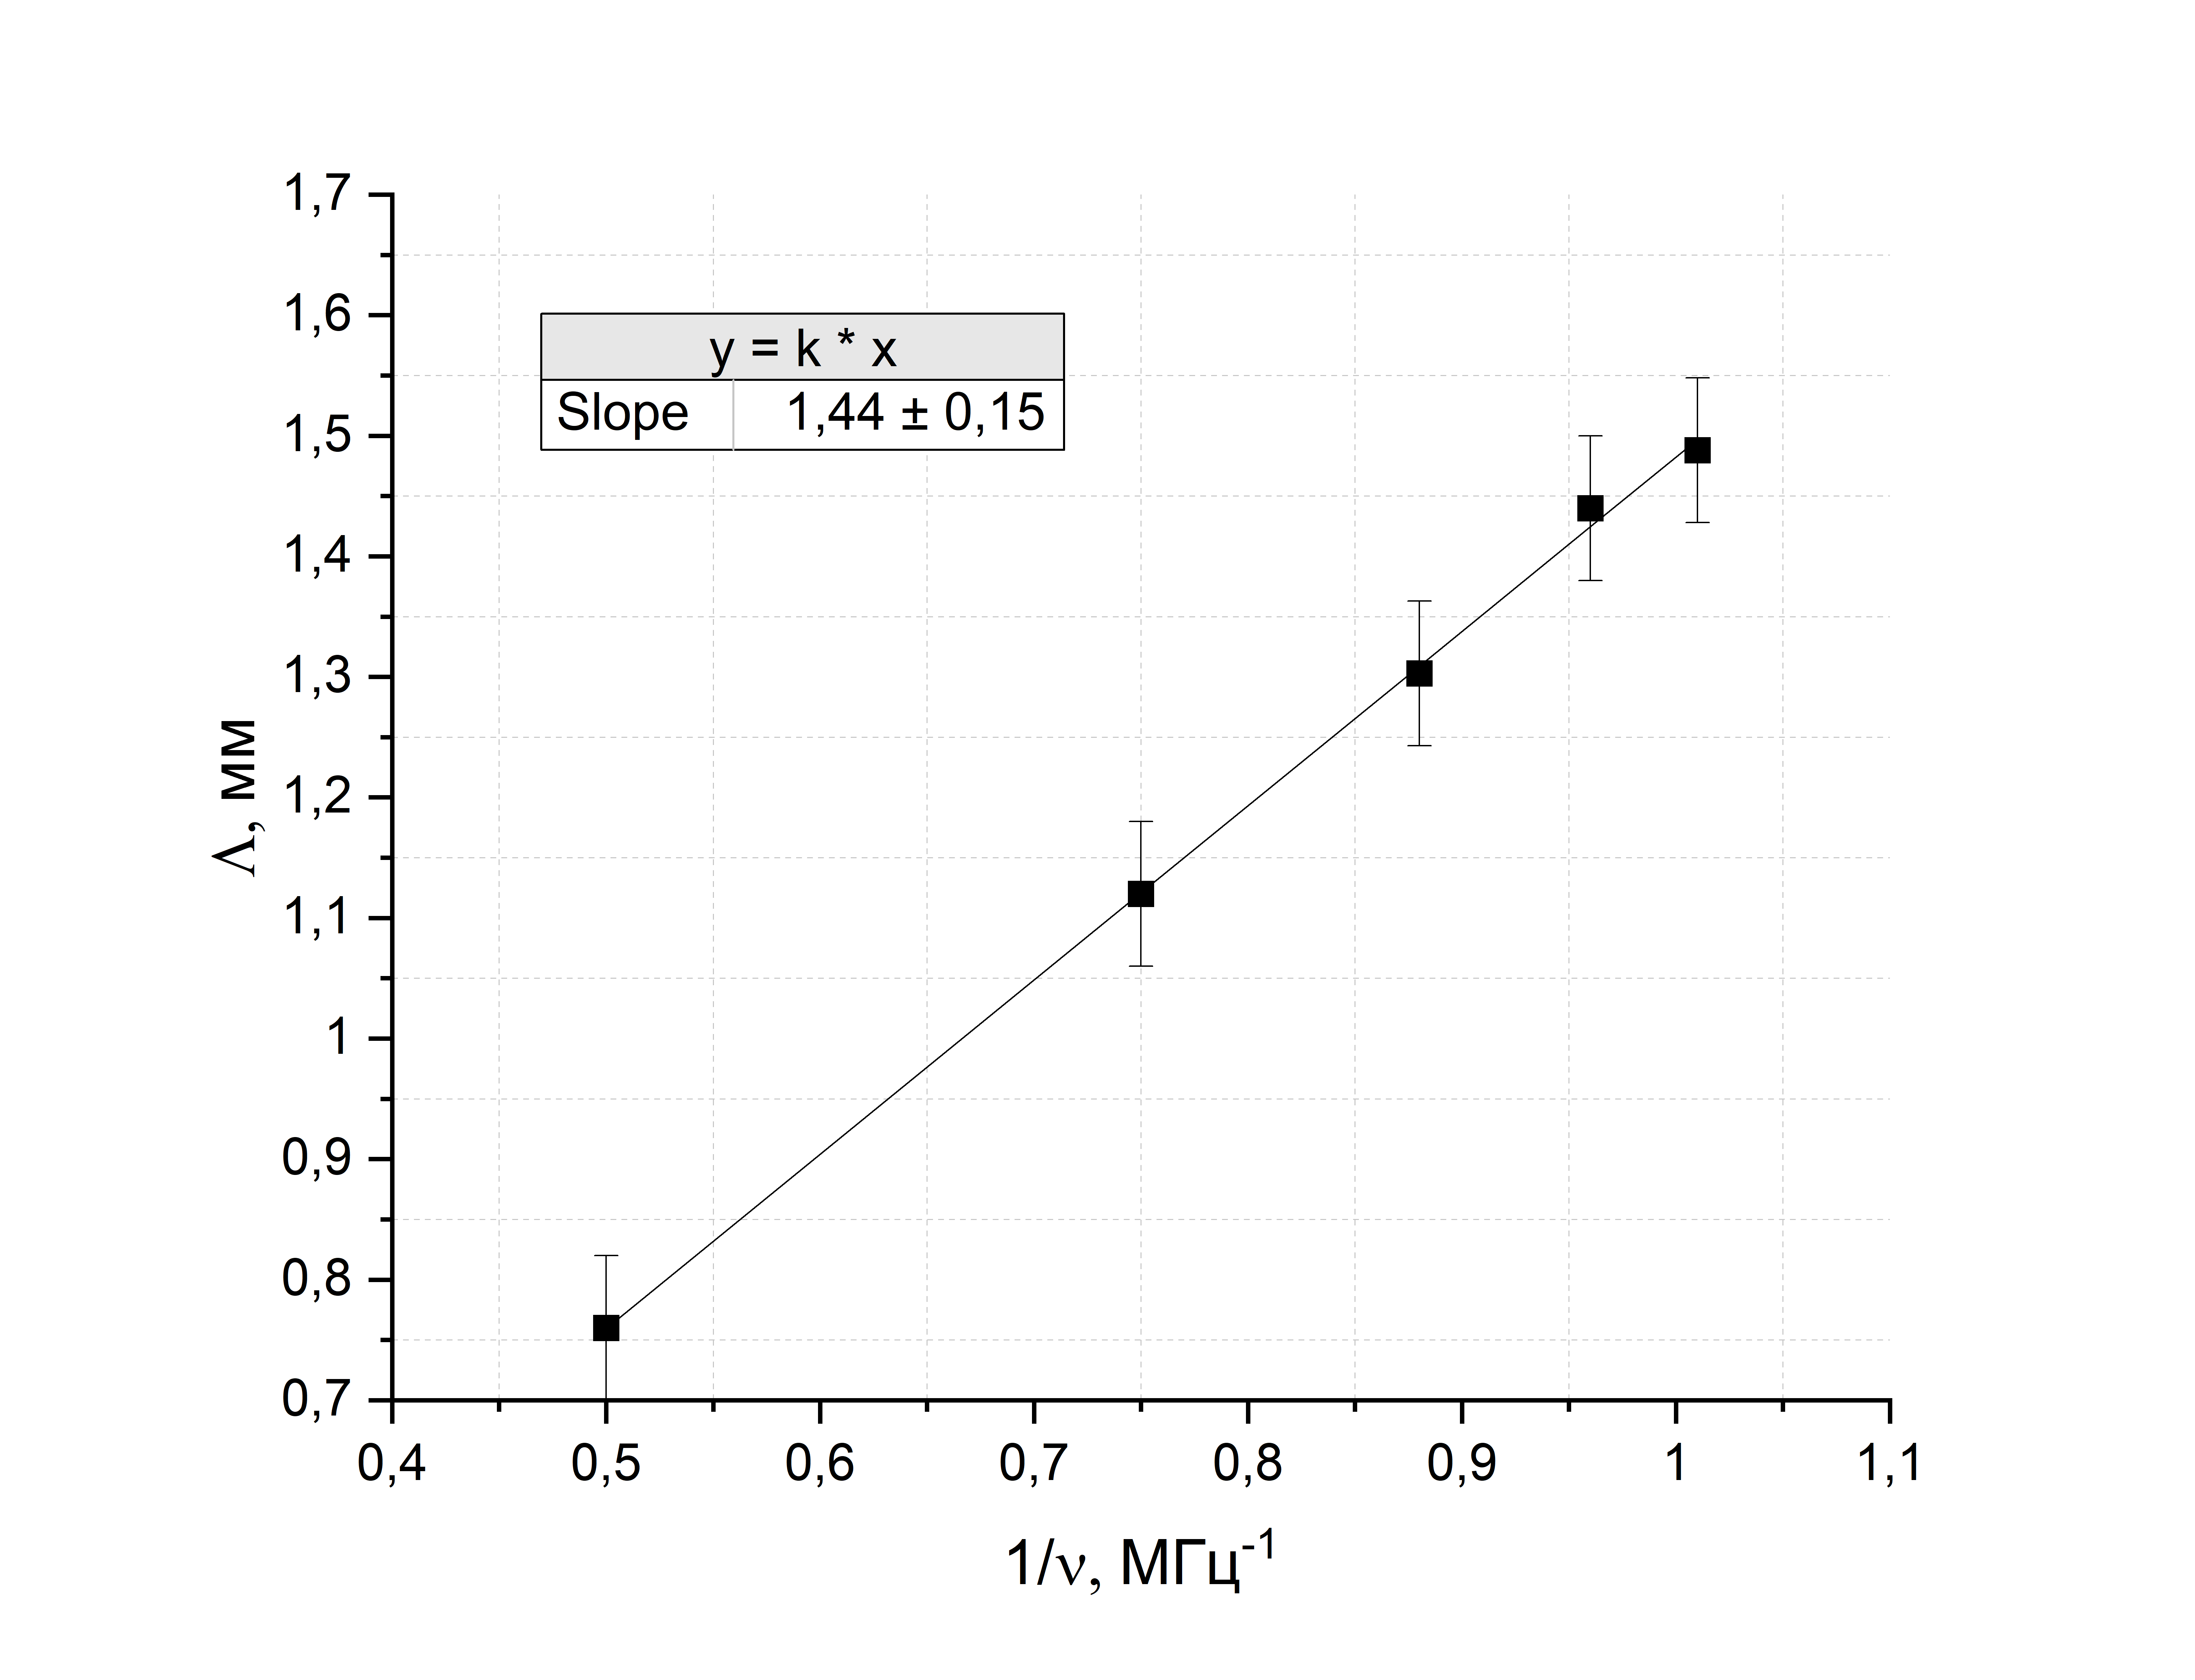
\includegraphics[width=0.8\textwidth]{v.png}
    \end{center}
    \caption{$\Lambda=F(1/\nu)$}
\end{figure}


%%%%%%%%%%%%%%%%%%%%%%%%%%%%%%%%%%%%%%%%%%%%%%%%%%%%%%%%%%%%%%%%%%%%%%%%%
 \section{Выводы}
\begin{enumerate}
    \item В работе была изучена дифракция на акустической решетке, создаваемой УЗ-волнами в воде
    \item По дифракционной картине были расчитаны длины УЗ-волн в воде для определенных частот
    \item С помощью метода темного поля было возможно пронаблюдать фазовую решетку, закрыв нулевой максимум дифракционной картины
    \item По взаимному расположению полос была рссчитана скорость звука в воде, совпадающая с ожидаемой в пределах погрешности

\end{enumerate}

\end{document}
